\documentclass[svgnames,11pt]{beamer}
\input{/home/tof/Documents/Cozy/latex-include/preambule_commun.tex}
\input{/home/tof/Documents/Cozy/latex-include/preambule_beamer.tex}
\usepackage{pgfpages} \setbeameroption{show notes on second screen=left}
\author[]{Christophe Viroulaud}
\title{Image numérique}
\date{\framebox{\textbf{Phot 01}}}
%\logo{}
\institute{Seconde - SNT}

\begin{document}
\begin{frame}
    \titlepage
\end{frame}
\begin{frame}
    \frametitle{}

    Le premier appareil photographique numérique semble avoir été commercialisé en 1981 (Sony). Depuis la photographie numérique n’a cessé de progresser pour pratiquement remplacer l’argentique.
    \begin{center}
        \centering
        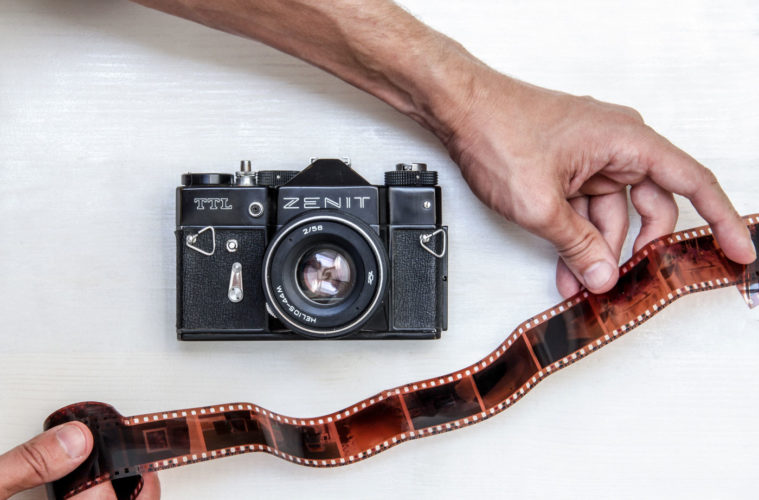
\includegraphics[width=7cm]{ressources/argentique.jpg}
        \captionof{figure}{Appareil photo argentique et sa pellicule}
        \label{IMG}
    \end{center}

\end{frame}
\begin{frame}
    \frametitle{}

    \begin{center}
        \framebox{Comment stocker une image dans un ordinateur?}
    \end{center}

\end{frame}
\section{Information discrète}
\subsection{Principe de l'argentique}
\begin{frame}
    \frametitle{Principe de l'argentique}
    Une pellicule est un film plastique recouvert de composés chimiques qui réagissent à la lumière.
    \begin{center}
        \centering
        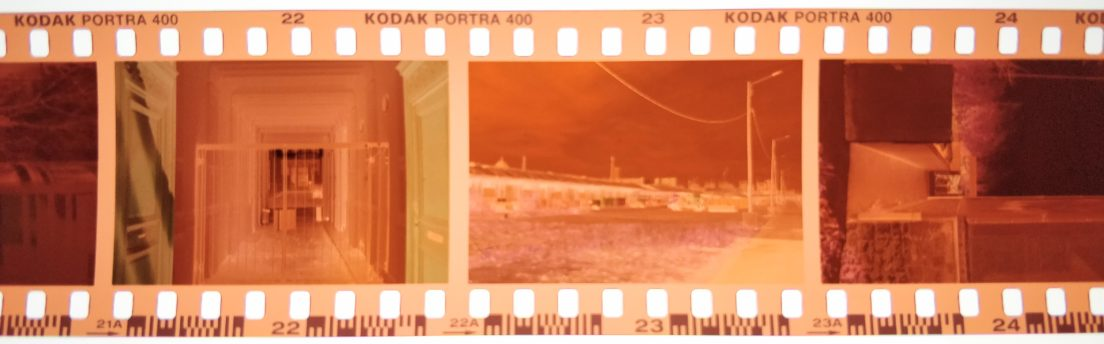
\includegraphics[width=6cm]{ressources/pellicule.jpg}
        \captionof{figure}{Pellicule argentique}
        \label{IMG}
    \end{center}
    \begin{aretenir}[]
        Dans une photographie argentique, les informations de l'image sont \textbf{continues}.
    \end{aretenir}
\end{frame}
\subsection{Principe du numérique}
\begin{frame}
    \frametitle{Principe du numérique}
    La mémoire d'un ordinateur est limitée.
    \begin{center}
        \centering
        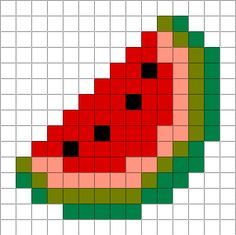
\includegraphics[width=4cm]{ressources/pasteque.jpg}
        \captionof{figure}{ Dans un ordinateur, une image est découpée en petits morceaux.}
        \label{IMG}
    \end{center}
    \begin{aretenir}[]
        Une image numérique est découpée en \textbf{pixels}. L'information de chaque pixel est une donnée \textbf{discrète}.
    \end{aretenir}
\end{frame}
\begin{frame}
    \frametitle{}

    \begin{center}
        \centering
        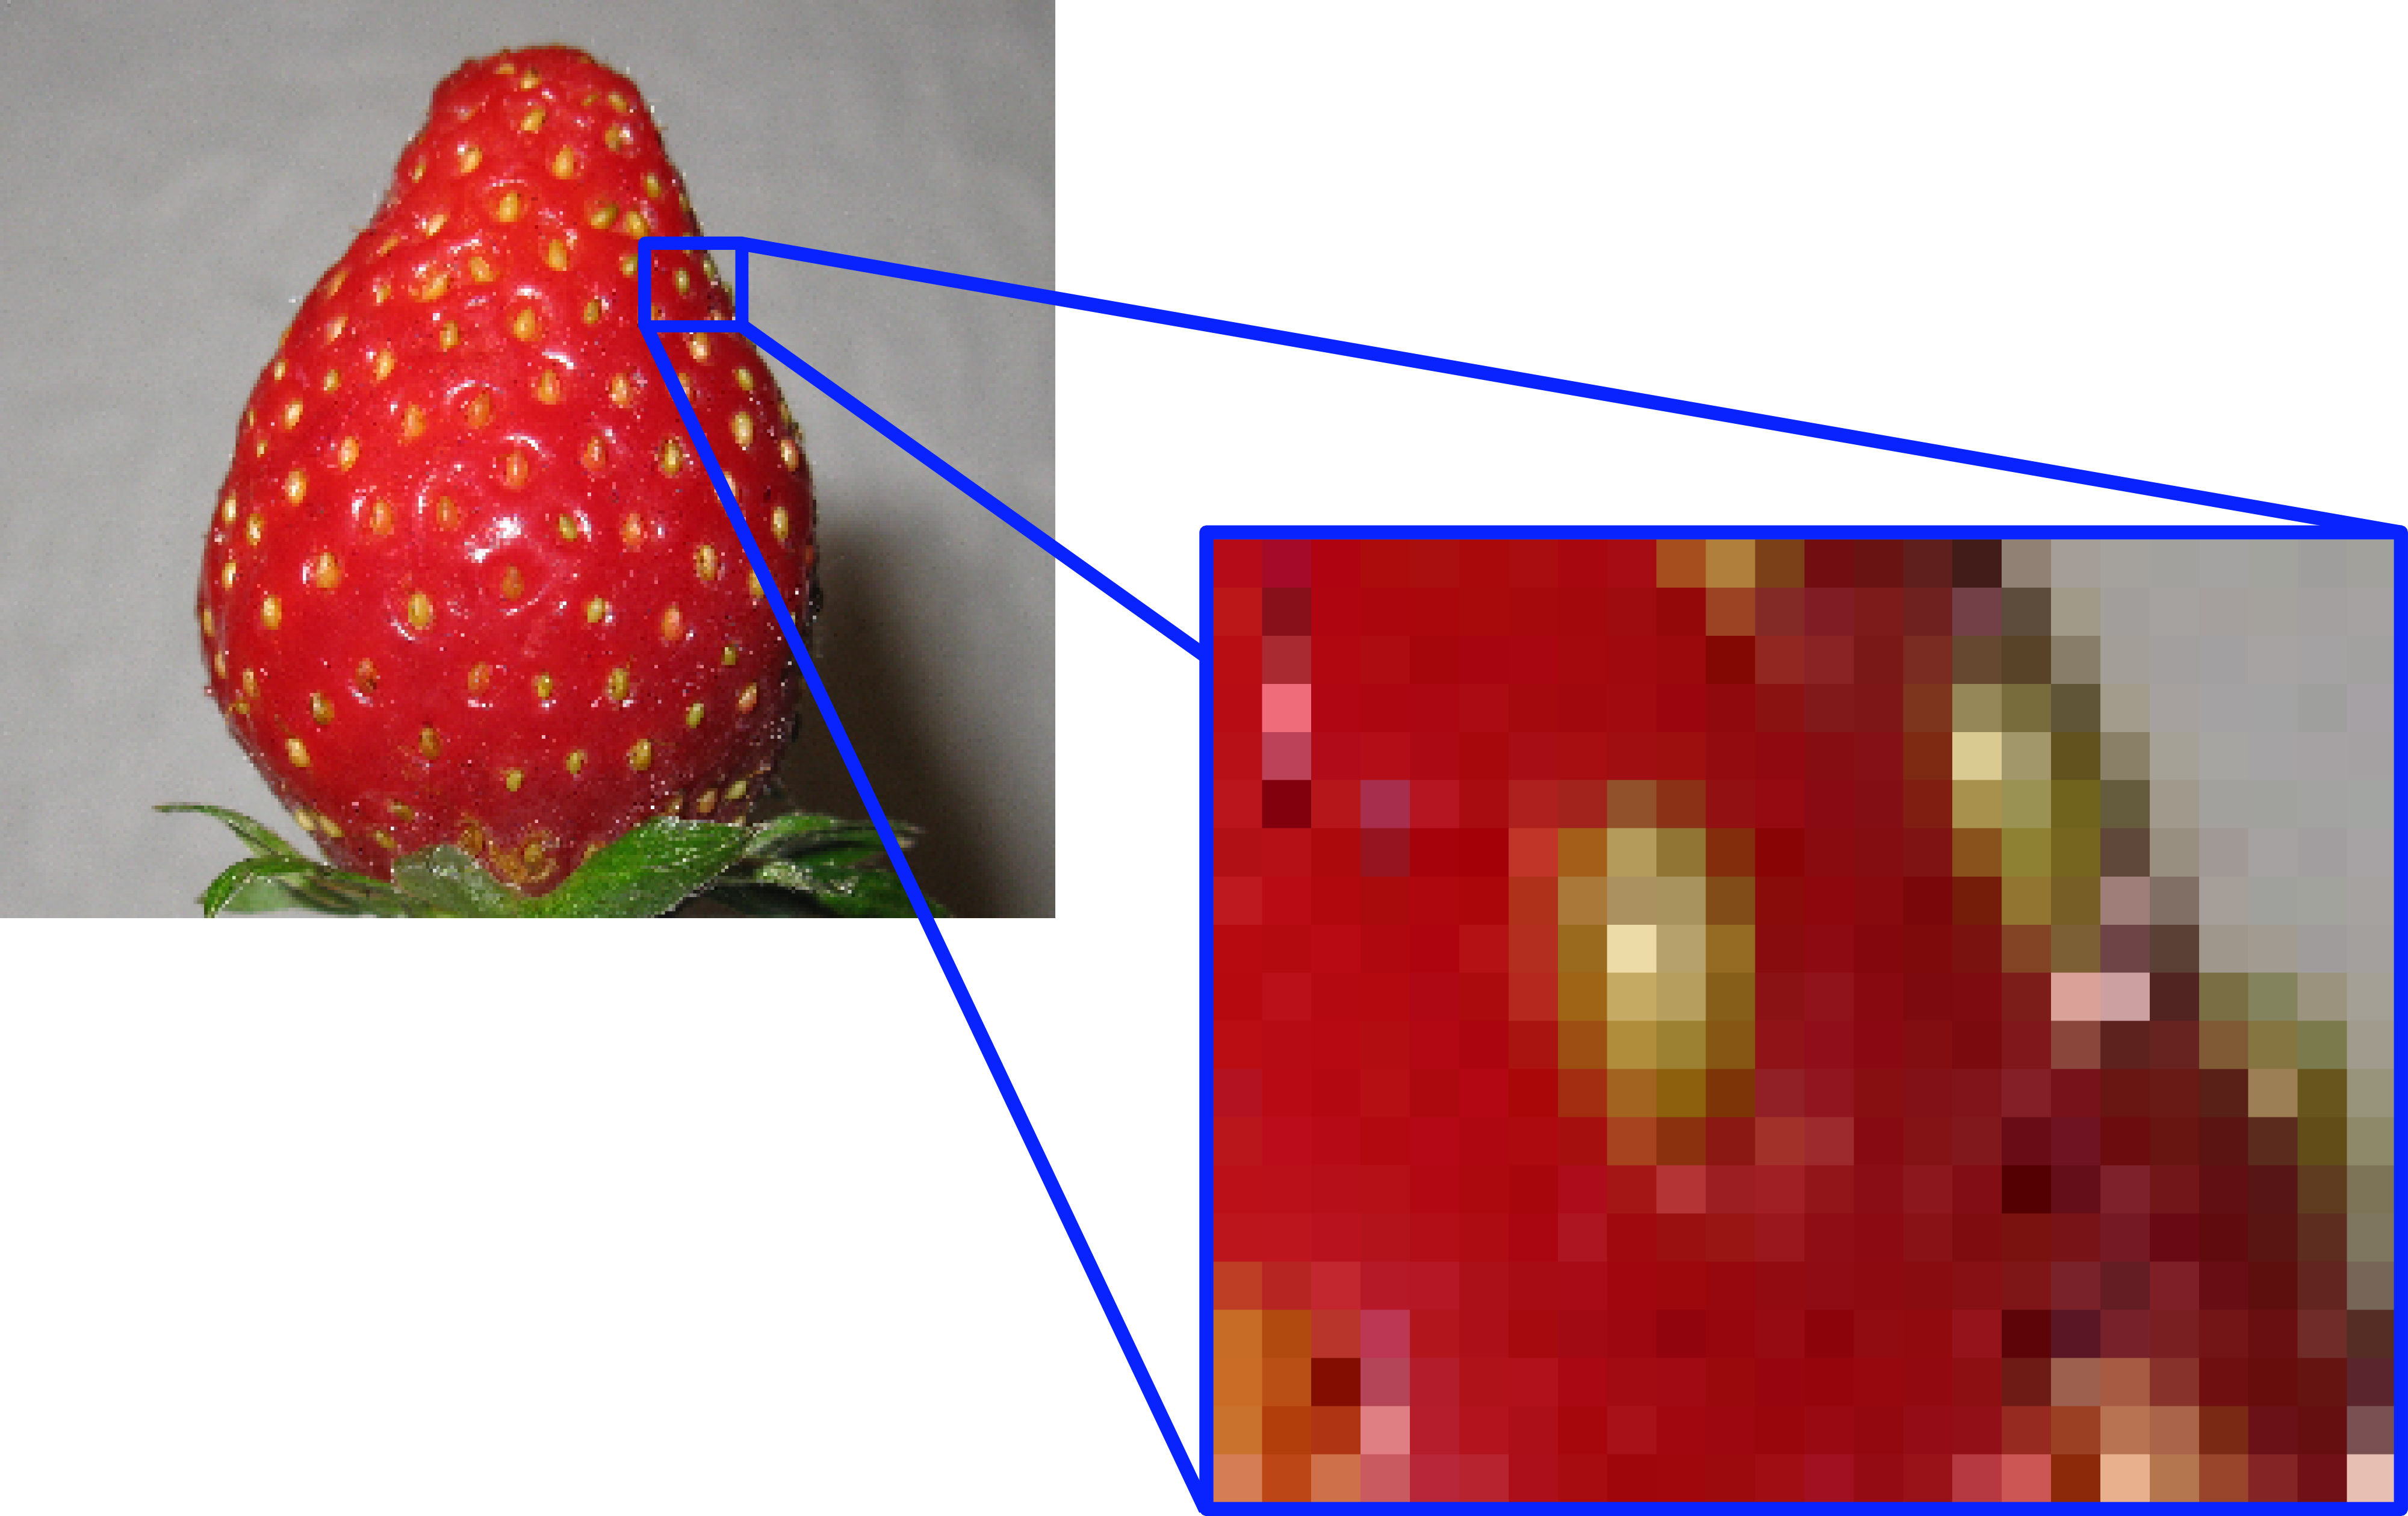
\includegraphics[width=9cm]{ressources/fraise.png}
        \captionof{figure}{L'ensemble des pixels crée une illusion de continuité}
        \label{IMG}
    \end{center}

\end{frame}
\begin{frame}
    \frametitle{}

    \begin{center}
        \centering
        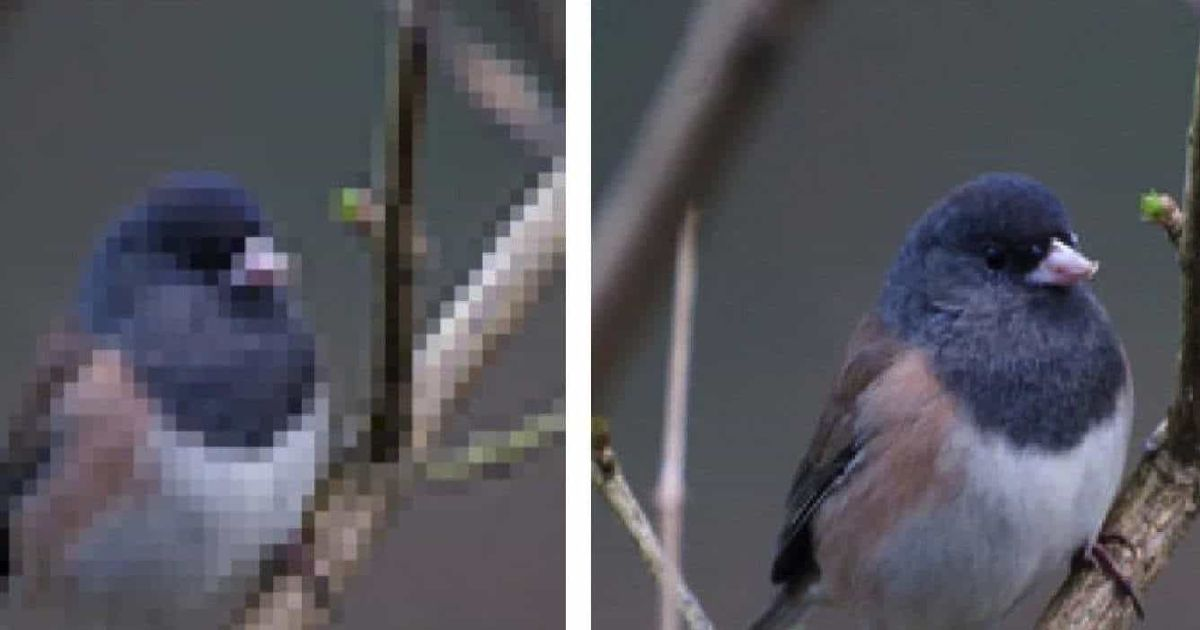
\includegraphics[width=9cm]{ressources/pixelisee.jpg}
        \captionof{figure}{Plus il y a de pixels plus il y a d'informations.}
        \label{IMG}
    \end{center}

\end{frame}
\section{Caractéristiques d'une image numérique}
\subsection{Dimensions}
\begin{frame}
    \frametitle{Dimensions d'une image numérique}
    \begin{center}
        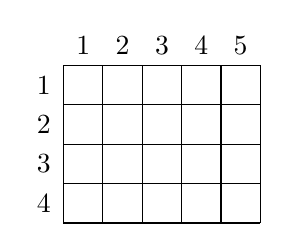
\begin{tikzpicture}[scale=0.5]
            \draw (0,0) grid (5,4);

            \draw (-0.5,3.5) node{1};
            \draw (-0.5,2.5) node{2};
            \draw (-0.5,1.5) node{3};
            \draw (-0.5,0.5) node{4};
            \draw (0.5,4.5) node{1};
            \draw (1.5,4.5) node{2};
            \draw (2.5,4.5) node{3};
            \draw (3.5,4.5) node{4};
            \draw (4.5,4.5) node{5};
        \end{tikzpicture}
        \label{matrice}
    \end{center}
    \begin{itemize}
        \item<1-> La \textbf{définition} d'une image de \emph{m} lignes et \emph{n} colonnes est $m×n$. L'image a une définition de $5×4=20~pixels$.
        \item<2-> La \textbf{résolution} est le nombre de pixels par unité de longueur. On utilise couramment l'unité américaine (le \emph{pouce}).
        \item<3-> Il existe plusieurs \textbf{formats} d'image: \emph{bitmap (bmp)}, \emph{jpeg} (Joint Photographic Experts Group) ou \emph{png} (Portable Network Graphics).
    \end{itemize}
    \note[item]{L'écran affiche une résolution de 72ppp (pixels par pouce).}
    \note[item]{en anglais: ppi pixel per inch ou dpi (density per inch)}
    \note[item]{nouveau format webp dvp par google; performance de compression > 30\% par rapport à jpg; pour diminuer quantité de données qui transitent sur le web (60\% d'images)}
\end{frame}
\begin{frame}
    \frametitle{}

    \begin{activite}
        \begin{center}
            \centering
            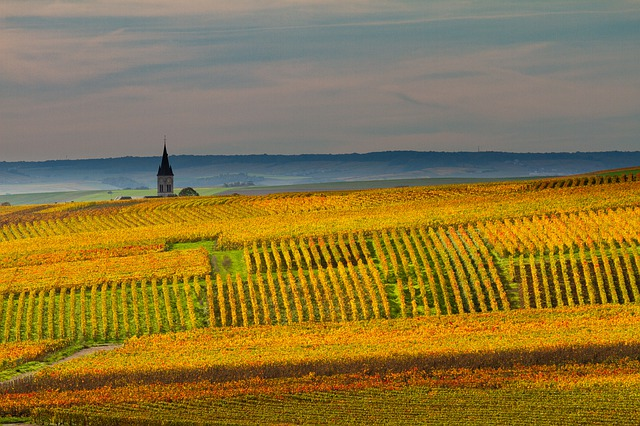
\includegraphics[width=4cm]{ressources/vigne.jpg}
            \captionof{figure}{Cette image possède 4000 colonnes et 3000 lignes.}
            \label{IMG}
        \end{center}
        \begin{enumerate}
            \item Calculer sa définition en pixels. La convertir en mégapixels.
            \item Sachant que:
                  \begin{itemize}
                      \item la résolution de l'image est 72ppp,
                      \item $1~pouce = 2,54cm$.
                  \end{itemize}
                  Calculer la longueur et la largeur réelle de l'image en centimètres.
        \end{enumerate}
    \end{activite}

\end{frame}
\begin{frame}
    \frametitle{Correction}

    $$4000×3000=12000000$$
    \begin{center}
        12 millions de pixels $\rightarrow$ 12 mégapixels
    \end{center}

\end{frame}
\begin{frame}[fragile]
    \frametitle{Correction}
    Longueur de l'image:
    \begin{center}
        \begin{tabular}{|*{3}{c|}}
            \hline
            pixels & 72 & 4000 \\
            \hline
            pouces & 1  & ?    \\
            \hline
        \end{tabular}
    \end{center}
    $$\frac{1×4000}{72}=55,6\mbox{ pouces}$$
    \begin{center}
        \begin{tabular}{|*{3}{c|}}
            \hline
            cm     & 2,54 & ?    \\
            \hline
            pouces & 1    & 55,6 \\
            \hline
        \end{tabular}
    \end{center}
    $$\frac{55,6×2,54}{1}=141\mbox{ cm}$$
\end{frame}
\subsection{Couleurs}
\subsubsection{Synthèse additive}
\begin{frame}
    \frametitle{Synthèse additive}
    \begin{aretenir}[]
        À partir de trois sources lumineuses primaires (\emph{Rouge, Vert, Bleu - RVB ou RGB en anglais}) il est possible d'obtenir une grande variété d'autres couleurs.
    \end{aretenir}

    \begin{activite}
        \begin{enumerate}
            \item Se rendre sur le site \url{https://tinyurl.com/addcol}
            \item Faire varier les curseurs pour ajouter ou supprimer une des trois couleurs.
        \end{enumerate}
    \end{activite}
\end{frame}
\begin{frame}
    \frametitle{}

    \begin{center}
        \centering
        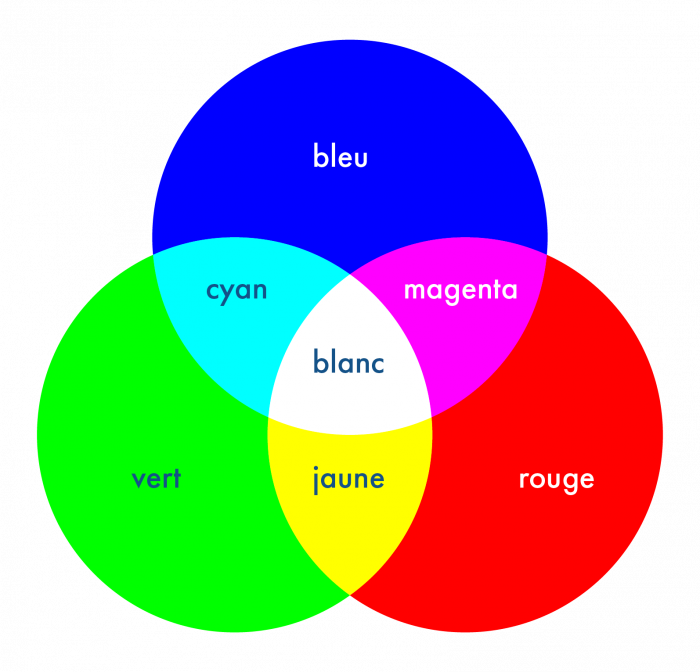
\includegraphics[width=8cm]{ressources/synthese-add.png}
        \captionof{figure}{Selon l'intensité des couleurs primaires on obtient une palette très variée.}
        \label{IMG}
    \end{center}

\end{frame}
\begin{frame}
    \frametitle{}

    \begin{activite}
        \begin{enumerate}
            \item Se rendre sur la page \url{https://htmlcolorcodes.com/fr/}.
            \item Dans le cadre de droite modifier les valeurs R G B au hasard.
            \item Quelles sont les valeurs minimale et maximale?
            \item Le \# indique la représentation \textbf{hexadécimale} d'une couleur. Quelle est la représentation du rouge primaire? Celle du vert?
        \end{enumerate}
    \end{activite}

\end{frame}
\begin{frame}
    \frametitle{Correction}

    \begin{itemize}
        \item Chaque couleur peut varier de 0 à 255 soit 256 valeurs.
              \begin{aretenir}[]
                  Avec ce système on peut créer $256×256×256=16777216$, soit plus de 16 millions de couleurs.
              \end{aretenir}
        \item Les couleurs:
              \begin{itemize}
                  \item rouge: \#FF0000
                  \item vert: \#00FF00
                  \item bleu: \#0000FF
              \end{itemize}
    \end{itemize}

\end{frame}
\begin{frame}
    \frametitle{}

    \begin{activite}
        \begin{enumerate}
            \item Dans le cadre de droite modifier les valeurs RGB:
                  \begin{itemize}
                      \item R 128
                      \item G 128
                      \item B 128
                  \end{itemize}
                  Quelle couleur obtient-on?
            \item Utiliser maintenant la combinaison (200, 200, 200). Quelles couleurs obtient-on quand les trois valeurs sont identiques?
            \item Comment obtient-on du blanc? du noir?
            \item Combien de niveaux de gris peut-on réaliser?
        \end{enumerate}
    \end{activite}

\end{frame}
\begin{frame}
    \frametitle{Correction}

    \begin{itemize}
        \item Quand les trois couleurs ont la même valeur on obtient du gris.
        \item On peut obtenir 256 niveaux de gris (blanc et noir inclus).
    \end{itemize}

\end{frame}
\begin{frame}
    \frametitle{Résumons}

    \begin{aretenir}[]
    \begin{itemize}
        \item Une image numérique peut contenir plusieurs millions de pixels.
        \item Chaque pixel est une couleur parmi plus de 16 millions possibles.
    \end{itemize}
    \end{aretenir}
\begin{center}
\centering

\includegraphics[width=4cm]{ressources/licorne.jpg}
\end{center}
\end{frame}
\subsubsection{Synthèse soustractive}
\begin{frame}
    \frametitle{Synthèse soustractive}

    Une imprimante à jet d'encre utilise quatre encres: \emph{Cyan, Magenta, Jaune, Noir}. En appliquant les trois premières couleurs sur une feuille blanche il est possible de créer les autres nuances par \emph{synthèse soustractive}.

\end{frame}
\begin{frame}
    \frametitle{}
    \begin{activite}
        \begin{enumerate}
            \item Convertir le nom des couleurs en anglais.
            \item Sur le site \url{https://htmlcolorcodes.com/fr/} obtenir le noir en utilisant les couleurs Cyan, Magenta, Jaune.
            \item Puisqu'il est possible d'obtenir le noir en combinant les trois couleurs, quel est l'intérêt de rajouter une cartouche d'encre noir dans l'imprimante?
        \end{enumerate}
    \end{activite}


\end{frame}
\begin{frame}
    \frametitle{Correction}

On utilise généralement beaucoup de noir lors d'une impression. Il est plus économique d'utiliser une cartouche spécifique plutôt que de mélanger trois couleurs.

\end{frame}
\end{document}